\section{Mössbauer Effect}

\frame[plain]{\tableofcontents[currentsection]}

\subsection{Definition}
	\begin{frame}
		\frametitle{Photon absorption by atoms}
		Nucleus can undergo transitions between quantum states like electrons in an atom.
		
		\begin{figure}
			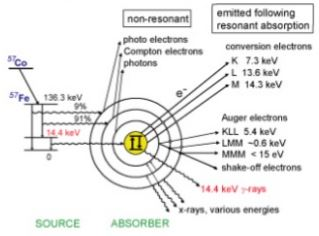
\includegraphics[width=7cm]{images/nuclear-excitations.jpg}
			\credit{University of Cyprus \cite{web:mossbauer6}}
			\caption{Absorption of photons by an atom}
		\end{figure}
	\end{frame}

	\begin{frame}
		\frametitle{Absorption and emission of $\gamma$-rays}
		Nucleus releases $\gamma$-ray with transition energy $E_0$. $\gamma$ doesn't carry full energy ($E_{\gamma} \neq E_0$), part is lost to recoil (momentum conservation).
		\begin{columns}
			\begin{column}{0.53\textwidth}
				\begin{figure}
					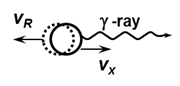
\includegraphics[width=3cm]{images/decay.png}
					{\color{black} \credit{Yi-Long Chen: Mössbauer Effect \cite{longyang07}}}
					\caption{Nucleus recoil ($\gamma$-ray emission)}
				\end{figure}
			\end{column}
		
			\begin{column}{0.43\textwidth}
				\begin{figure}
					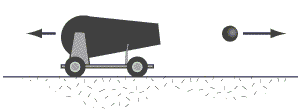
\includegraphics[width=3cm]{images/recoil-gun.png}
					\credit{St. Mary's H.S. Physics \cite{web:stmaryhs}}
					\caption{Gun recoil}
				\end{figure}
			\end{column}
		\end{columns}
	
		\begin{block}{Momentum/energy conservation}
			\fontsize{9.5pt}{12pt}
			\begin{columns}
				\begin{column}[T]{0.4\linewidth}
					\begin{equation*}
						\begin{cases}
							Mv_x&=\frac{E_{\gamma}}{c} + M(v_x-v_R)\\
							E_e+\frac{1}{2}Mv_x^2&=E_g+E_{\gamma}+\frac{1}{2}M(v_x-v_R)^2
						\end{cases}
					\end{equation*}
				\end{column}
				\begin{column}[T]{0.55\linewidth}
					\begin{description}
						\item [$v_x$, $v_R$] initial/recoil velocity
						\item [$E_g$, $E_e$] ground/excited state energy
					\end{description}
				\end{column}
			\end{columns}
		\end{block}
	\end{frame}
	
	\begin{frame}
		\frametitle{Gamma Decay}
	
		\begin{block}{Energy of $\gamma$-ray}
			\fontsize{9.5pt}{12pt}
			\begin{equation*}
				E_{\gamma}=E_0-E_R+E_D, \quad \underbrace{E_R=\frac{1}{2}Mv_R^2=\frac{E_{\gamma}^2}{2Mc^2}}_{\text{recoil energy}}, \quad
				\underbrace{E_D=Mv_xv_R=\frac{v_x}{c}E_{\gamma}}_{\text{Doppler energy shift}}
			\end{equation*}
			\begin{description}
				\item [$E_0=E_e-E_g$] energy difference between excited and ground state
			\end{description}
		\end{block}
	
		\begin{columns}
			\begin{column}{0.4\linewidth}
				\begin{block}{Energy-time uncertainty}
					\centering
					$\Delta E \cdot \Delta t \geq \frac{\hbar}{2}$
				\end{block}
				\begin{block}{Example for $\ce{^{57}Fe}$}
					\centering
					$E_0=\unit[14.4]{keV}$\\
					$\tau=\unit[141.1]{ns}$\\
					$\Gamma_n=\unit[4.66 x 10^{-9}]{eV}$
				\end{block}
			\end{column}
			\begin{column}{0.55\linewidth}
				\begin{block}{Natural line width $\Gamma_n$}
					\centering
					Stability of an energy level: $\Gamma_n \tau \geq \hbar / 2$
					\begin{enumerate}
						\item[$\tau$] energy level lifetime (typically $\unit[10^{-10}]{s}$ for nuclear transitions)
					\end{enumerate}
				\end{block}
			\end{column}
		\end{columns}
	
	\end{frame}
	
	\begin{frame}[t]
		\frametitle{Nuclear resonant absorption}
		
		\begin{figure}
			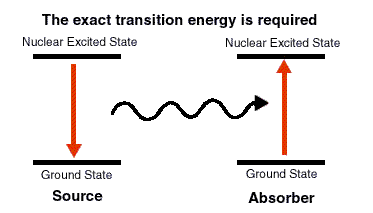
\includegraphics[width=6cm]{images/transition.png}
			\credit{Georgia State University \cite{web:mossbauergsu}}
		\end{figure}
		
		\begin{columns}
			\begin{column}{0.48\linewidth}
				\begin{block}{Energy needed for absorption}
					\begin{eqnarray*}
						E_{\gamma}^{abs.}&=E_0 + 2 \cdot E_R\\
						&=E_0 + \frac{E_{\gamma}^2}{Mc^2}
					\end{eqnarray*}
				\end{block}
			\end{column}
		\end{columns}
		
	\end{frame}

	\begin{frame}
		\frametitle{Nuclear resonant absorption}
		\begin{block}{$v_x=0 \Rightarrow E_D=0$}
			\begin{figure}
				\centering
				\resizebox{.5\textwidth}{!}{%
					\centering
\sansmath
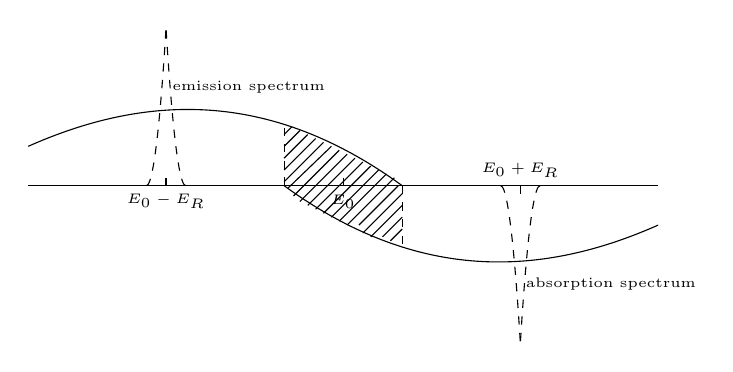
\begin{tikzpicture}
	\draw (0,5) -- (8,5);
	\path [black,bend left,-,] (0,5.5) edge (4.75,5);
	\path [black,bend left,-,] (8,4.5) edge (3.25,5);
	\draw[black,dashed] (4.75,5) -- (4.75,4.25);
	\draw[black,dashed] (3.25,5) -- (3.25,5.75);
	\draw (4,5) -- (4,5.1);
	\node at (4,4.8) {\tiny $E_0$};
	\draw (1.75,5) -- (1.75,5.1);
	\node at (1.75,4.8) {\tiny $E_0-E_R$};
	\draw (6.25,5) -- (6.25,4.9);
	\node at (6.25,5.2) {\tiny $E_0+E_R$};
	\draw[dashed] (1.5,5) parabola (1.75,7);
	\draw[dashed] (2,5) parabola (1.75,7);
	\draw[dashed] (6,5) parabola (6.25,3);
	\draw[dashed] (6.5,5) parabola (6.25,3);
	\node at (2.8,6.25) {\tiny emission spectrum};
	\node at (7.4,3.75) {\tiny absorption spectrum};
	\draw (3.25,5.65) -- (3.35,5.75);
	\draw (3.25,5.5) -- (3.45,5.7);
	\draw (3.25,5.35) -- (3.55,5.65);
	\draw (3.25,5.2) -- (3.65,5.6);
	\draw (3.25,5.05) -- (3.75,5.55);
	\draw (3.3,4.97) -- (3.85,5.5);
	\draw (3.37,4.87) -- (3.95,5.45);
	\draw (3.45,4.8) -- (4.05,5.4);
	\draw (3.55,4.75) -- (4.15,5.35);
	\draw (3.65,4.7) -- (4.25,5.3);
	\draw (3.75,4.65) -- (4.35,5.25);
	\draw (3.85,4.6) -- (4.45,5.2);
	\draw (3.95,4.55) -- (4.55,5.15);
	\draw (4.05,4.5) -- (4.65,5.1);
	\draw (4.2,4.5) -- (4.7,5);
	\draw (4.25,4.4) -- (4.75,4.9);
	\draw (4.35,4.35) -- (4.75,4.75);
	\draw (4.5,4.35) -- (4.75,4.6);
	\draw (4.6,4.3) -- (4.75,4.45);
\end{tikzpicture}
				}
				\credit{Yi-Long Chen: Mössbauer Effect \cite{longyang07}}
				\caption{Emission and absorption $\gamma$-ray spectra with recoil \cite{longyang07}}
			\end{figure}
		\end{block}
	
		\begin{columns}
			\begin{column}{0.48\textwidth}
				\begin{block}{Spectrum (dashed line)}
					\begin{itemize}
						\item sharp peaks centered
						\item full-width at half-maximum (FWHM) $\approx \Gamma_n$
					\end{itemize}
				\end{block}
			\end{column}
		
			\begin{column}{0.48\textwidth}
				\begin{block}{Resonant absorption condition}
					\centering
					\begin{equation*}
						\frac{\Gamma_n}{2E_R}>1
					\end{equation*}
				\end{block}
			\end{column}
		\end{columns}
		
	\end{frame}
	
	\begin{frame}
		\frametitle{Nuclear resonant absorption}
		\begin{block}{$v_x \neq 0 \Rightarrow E_D \neq 0$}
			\begin{figure}
				\centering
				\resizebox{.4\textwidth}{!}{%
					\centering
\sansmath
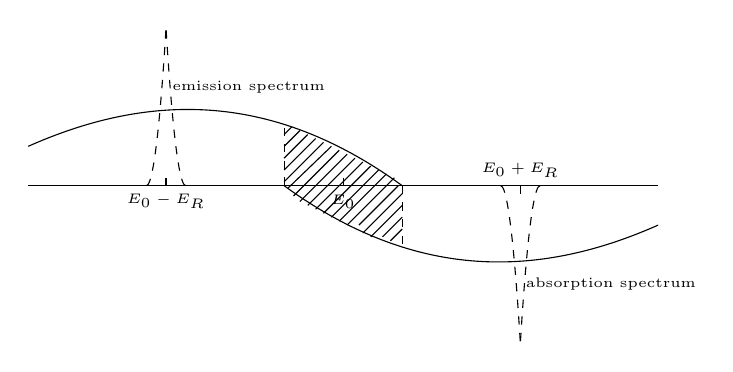
\begin{tikzpicture}
	\draw (0,5) -- (8,5);
	\path [black,bend left,-,] (0,5.5) edge (4.75,5);
	\path [black,bend left,-,] (8,4.5) edge (3.25,5);
	\draw[black,dashed] (4.75,5) -- (4.75,4.25);
	\draw[black,dashed] (3.25,5) -- (3.25,5.75);
	\draw (4,5) -- (4,5.1);
	\node at (4,4.8) {\tiny $E_0$};
	\draw (1.75,5) -- (1.75,5.1);
	\node at (1.75,4.8) {\tiny $E_0-E_R$};
	\draw (6.25,5) -- (6.25,4.9);
	\node at (6.25,5.2) {\tiny $E_0+E_R$};
	\draw[dashed] (1.5,5) parabola (1.75,7);
	\draw[dashed] (2,5) parabola (1.75,7);
	\draw[dashed] (6,5) parabola (6.25,3);
	\draw[dashed] (6.5,5) parabola (6.25,3);
	\node at (2.8,6.25) {\tiny emission spectrum};
	\node at (7.4,3.75) {\tiny absorption spectrum};
	\draw (3.25,5.65) -- (3.35,5.75);
	\draw (3.25,5.5) -- (3.45,5.7);
	\draw (3.25,5.35) -- (3.55,5.65);
	\draw (3.25,5.2) -- (3.65,5.6);
	\draw (3.25,5.05) -- (3.75,5.55);
	\draw (3.3,4.97) -- (3.85,5.5);
	\draw (3.37,4.87) -- (3.95,5.45);
	\draw (3.45,4.8) -- (4.05,5.4);
	\draw (3.55,4.75) -- (4.15,5.35);
	\draw (3.65,4.7) -- (4.25,5.3);
	\draw (3.75,4.65) -- (4.35,5.25);
	\draw (3.85,4.6) -- (4.45,5.2);
	\draw (3.95,4.55) -- (4.55,5.15);
	\draw (4.05,4.5) -- (4.65,5.1);
	\draw (4.2,4.5) -- (4.7,5);
	\draw (4.25,4.4) -- (4.75,4.9);
	\draw (4.35,4.35) -- (4.75,4.75);
	\draw (4.5,4.35) -- (4.75,4.6);
	\draw (4.6,4.3) -- (4.75,4.45);
\end{tikzpicture}
				}
				\credit{Yi-Long Chen: Mössbauer Effect \cite{longyang07}}
				\caption{Emission and absorption $\gamma$-ray spectra with recoil \cite{longyang07}}
			\end{figure}
		\end{block}
	
		\begin{block}{Spectrum}
			\begin{itemize}
				\item $FWHM \gg \Gamma$
				\item thermal random motion of atoms (Maxwell distribution of $v_x$): $p(v_x)dv_x=\left(\frac{M}{2 \pi k_B T} \right)^{\frac{1}{2}} exp\left(-\frac{M}{2 k_B T} v_x^2 \right) dv_x$
				\item width of Doppler broadening $\Delta E_D=4 \sqrt{E_R k_B T \ln{2}}$
			\end{itemize}
		\end{block}
	\end{frame}

	\begin{frame}
		\frametitle{Nuclear resonant absorption}
		\begin{block}{$v_x \neq 0 \Rightarrow E_D \neq 0$}
			\begin{figure}
				\centering
				\resizebox{.4\textwidth}{!}{%
					\centering
\sansmath
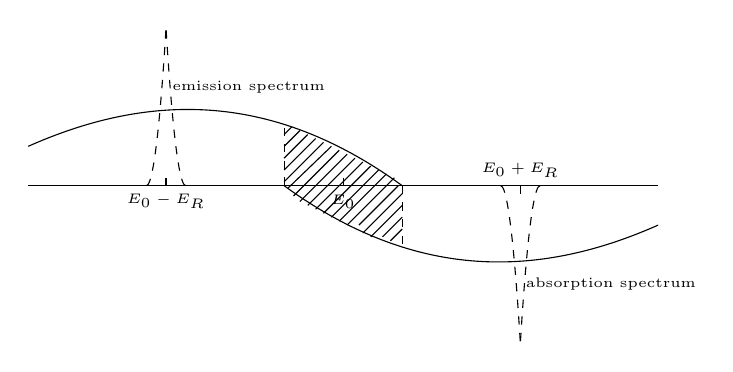
\begin{tikzpicture}
	\draw (0,5) -- (8,5);
	\path [black,bend left,-,] (0,5.5) edge (4.75,5);
	\path [black,bend left,-,] (8,4.5) edge (3.25,5);
	\draw[black,dashed] (4.75,5) -- (4.75,4.25);
	\draw[black,dashed] (3.25,5) -- (3.25,5.75);
	\draw (4,5) -- (4,5.1);
	\node at (4,4.8) {\tiny $E_0$};
	\draw (1.75,5) -- (1.75,5.1);
	\node at (1.75,4.8) {\tiny $E_0-E_R$};
	\draw (6.25,5) -- (6.25,4.9);
	\node at (6.25,5.2) {\tiny $E_0+E_R$};
	\draw[dashed] (1.5,5) parabola (1.75,7);
	\draw[dashed] (2,5) parabola (1.75,7);
	\draw[dashed] (6,5) parabola (6.25,3);
	\draw[dashed] (6.5,5) parabola (6.25,3);
	\node at (2.8,6.25) {\tiny emission spectrum};
	\node at (7.4,3.75) {\tiny absorption spectrum};
	\draw (3.25,5.65) -- (3.35,5.75);
	\draw (3.25,5.5) -- (3.45,5.7);
	\draw (3.25,5.35) -- (3.55,5.65);
	\draw (3.25,5.2) -- (3.65,5.6);
	\draw (3.25,5.05) -- (3.75,5.55);
	\draw (3.3,4.97) -- (3.85,5.5);
	\draw (3.37,4.87) -- (3.95,5.45);
	\draw (3.45,4.8) -- (4.05,5.4);
	\draw (3.55,4.75) -- (4.15,5.35);
	\draw (3.65,4.7) -- (4.25,5.3);
	\draw (3.75,4.65) -- (4.35,5.25);
	\draw (3.85,4.6) -- (4.45,5.2);
	\draw (3.95,4.55) -- (4.55,5.15);
	\draw (4.05,4.5) -- (4.65,5.1);
	\draw (4.2,4.5) -- (4.7,5);
	\draw (4.25,4.4) -- (4.75,4.9);
	\draw (4.35,4.35) -- (4.75,4.75);
	\draw (4.5,4.35) -- (4.75,4.6);
	\draw (4.6,4.3) -- (4.75,4.45);
\end{tikzpicture}
				}
				\credit{Yi-Long Chen: Mössbauer Effect \cite{longyang07}}
				\caption{Emission and absorption $\gamma$-ray spectra with recoil \cite{longyang07}}
			\end{figure}
		\end{block}
	
		\begin{block}{Example for $\ce{^{57}Fe}$}
			At $T=\unit[300]{K}$, $\Delta E_D=\unit[24]{meV} > 2 E_R=\unit[4]{meV}$
			\begin{itemize}
				\item[$\rightarrow$] small overlap between emission and absorption spectra
				\item[$\rightarrow$] non-zero probability for a resonant process
			\end{itemize}
			Shifting due to recoil, broadening due to thermal motion spectrum
		\end{block}
	\end{frame}

\subsection{Discovery and Historical Remarks}

	\begin{frame}
		\frametitle{Compensating for recoil energy}
		
		\begin{enumerate}
			\item Mechanical motion of the source
			\begin{itemize}
				\item source mounted on tip of high-speed rotor
				\item $\gamma$-rays gained extra energy
				\begin{equation*}
					\Delta E=\frac{v}{c} E_{\gamma}\quad \Rightarrow \quad \frac{v}{c}E_{\gamma}=2E_R
				\end{equation*}
				\begin{equation*}
					\text{(for } \ce{^{57}Fe} \text{, } v=\unit[81]{m/s}\approx\unit[292]{km/h} \text{)}
				\end{equation*}
			\end{itemize}
			\item Doppler broadening
			\begin{itemize}
				\item temperature increase $\Rightarrow$ overlapping emission and absorption spectra
			\end{itemize}
		\end{enumerate}
	
		\begin{block}{Limitations}
			\begin{enumerate}
				\item low count rate: $\gamma$-rays usable for very short periods
				\item maximum speed of mechanical rotor
				\item recoil still present
			\end{enumerate}
		\end{block}
		
	\end{frame}
	
	\begin{frame}
		\frametitle{Discovery}
		\begin{columns}
			\begin{column}{0.38\linewidth}
				\begin{figure}
					\centering
					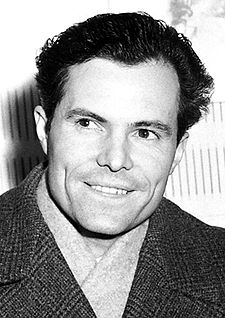
\includegraphics[width=3.5cm]{images/moessbauer-portrait.jpg}
					\credit{Wikipedia \cite{wiki:moessbauer}}
					\caption{Rudolph Mössbauer}
				\end{figure}
			\end{column}
			\begin{column}{0.58\linewidth}
				\textbf{Born:} January 31, 1929 (Munich) \\
				\textbf{Died:} September 14, 2011 (Grünwald)\vspace{\baselineskip}
				\textbf{1958} PhD on \textit{recoilless nuclear fluorescence of gamma rays in $^{191}\ce{Ir}$}
				\fontsize{9pt}{11pt}
				\begin{em}
					\flushright
					Z. Physik, \textbf{151}, 124 (1958)
					
					Naturwissenschaften \textbf{45}, 538 (1958)
					
					Z. Naturforsch. \textbf{14a}, 211 (1959)
					
				\end{em}
				\par
				\textbf{1961} Nobel Prize in Physics
				\fontsize{8pt}{9pt}
				\begin{quotation}
					\flushright
					''for his researches concerning the resonance absorption of gamma radiation and his discovery in this connection of the effect which bears his name''
				\end{quotation}
			\end{column}
		\end{columns}
	\end{frame}
		
	\begin{frame}
		\frametitle{Discovery}
		
		\fontsize{9.5pt}{10pt}
		\begin{block}{Mössbauer Experiment}
			\begin{itemize}
				\item source nuclei $\ce{^{191}Os}$, absorber nuclei $\ce{^{191}Ir}$, both heated at $\unit[88]{K}$
				\item both source and absorber rigidly bound in crystal latices
			\end{itemize}
		$\Rightarrow$ resonant absorption
		\end{block}
	
		\begin{columns}
			\begin{column}{0.49\linewidth}
				\begin{figure}
					\sansmath
					\centering
					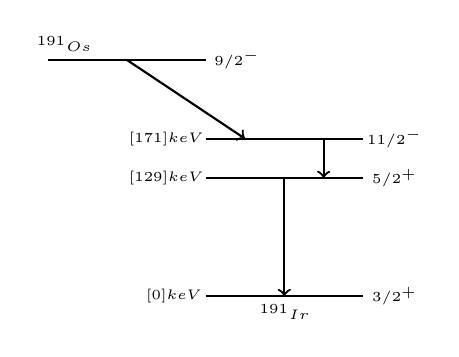
\begin{tikzpicture}[
						font=\sffamily,
						level/.style={black,thick}]
						\node at (0.2, 3.2) {\tiny $\ce{^{191}Os}$};
						\node at (3, -0.2) {\tiny $\ce{^{191}Ir}$};
						\node at (1.5, 2) {\tiny $\unit[171]{keV}$};
						\node at (1.5, 1.5) {\tiny $\unit[129]{keV}$};
						\node at (1.6, 0) {\tiny $\unit[0]{keV}$};
						\node at (2.4, 3) {\tiny $\text{9/2}^{-}$};
						\node at (4.4, 2) {\tiny $\text{11/2}^{-}$};
						\node at (4.4, 1.5) {\tiny $\text{5/2}^{+}$};
						\node at (4.4, 0) {\tiny $\text{3/2}^{+}$};
						\draw[thick] (0,3) -- (2,3);
						\draw[thick] (2,2) -- (4,2);
						\draw[thick] (2,1.5) -- (4,1.5);
						\draw[thick] (2,0) -- (4,0);
						\draw[thick,->] (1,3) -- (2.5,2);
						\draw[thick,->] (3.5,2) -- (3.5,1.5);
						\draw[thick,->] (3,1.5) -- (3,0);
					\end{tikzpicture}
					\credit{Yi-Long Chen: Mössbauer Effect \cite{longyang07}}
					\caption{Decay scheme of $\ce{^{191}Os}$ \cite{longyang07}}
				\end{figure}
			\end{column}
		
			\begin{column}{0.48\linewidth}
				\fontsize{9.5pt}{11pt}
				\begin{block}{Classical Explanation}
					\begin{itemize}
						\item atom held by $\unit[10]{eV}$ chemical bond energy in crystal lattice
						\item recoil energy for $\unit[129]{keV}$ photon in $\ce{^{191}Ir}$: $\unit{4.7 x 10^{-2}}{eV}$
					\end{itemize}
					$\Rightarrow$ recoil $\ll$ chemical bond energy\\
					$\Rightarrow$ entire lattice recoils ($\approx N_A$):
					$E_R=\frac{E_{\gamma}^2}{2Mc^2}=\unit[10^{-20}]{eV} \rightarrow \frac{\Gamma}{2R} > 1$
				\end{block}
			\end{column}
		\end{columns}
	\end{frame}
	
	\begin{frame}{Mössbauer Effect}
	
		\begin{block}{Spectrum}
			\begin{minipage}[t][.65\textheight][t]{.48\textwidth}
				\begin{figure}
					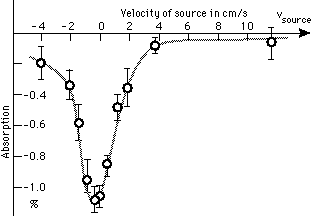
\includegraphics[width=5cm]{images/moessbauer-effect.png}
					\credit{Yi-Long Chen: Mössbauer Effect \cite{longyang07}}
					\caption{Resonance absorption curve of the $\unit[129]{keV}$ $\gamma$-rays by $\ce{^{191}Ir}$ \cite{web:mossbauertheory}}
				\end{figure}
			\end{minipage}
			\begin{minipage}[t][.65\textheight][c]{.48\textwidth}
				\begin{itemize}
					\item width $\Delta E =\unit[4.6 x 10^{-6}]{eV}$
					\item very high energy resolution $\frac{\Delta E}{E}=3.5 x 10^{-11}$
					\item $\Delta E \approx 2 \cdot \Gamma_N$
					\item Doppler effect modulates $\gamma$-ray energy to small energy range $E_{\gamma}(1 \pm v/c)$
				\end{itemize}
			\end{minipage}
		\end{block}
	
		$\Rightarrow$ \emph{new} opportunities for research (i.e. Zeeman effect first observed using the Mössbauer effect)	
	
	\end{frame}

	\begin{frame}
		\frametitle{Mössbauer Effect}
		\fontsize{9.5pt}{11pt}
		\begin{block}{Einstein Solid}
			Assumptions:
			\begin{itemize}
				\item lattice atoms are independent quantum harmonic oscillators
				\item same-frequency oscillation of atoms (unlike Debye model)
			\end{itemize}
		
			\begin{figure}
				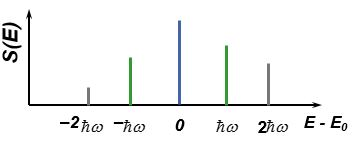
\includegraphics[width=5cm]{images/einstein-model.jpg}
				\caption{Einstein model of a solid}
			\end{figure}
		\end{block}
	
		\fontsize{9.5pt}{11pt}
		\begin{block}{Derivation of the effect}
			\begin{itemize}
				\item atoms bound in crystal lattice and vibrate about equilibrium position
				\item lattice vibrations are quantized: $E_p=\hbar \omega$
				\item photons exchange energy with lattice by creating/annihilating phonons
			\end{itemize}
		\end{block}
	
	\end{frame}
	
	\begin{frame}
		\frametitle{Mössbauer effect}
		\begin{block}{Lamb-Mössbauer (recoilless) factor}
			\begin{itemize}
				\item Condition for recoilless resonant absorption: $E_R \ll \hbar \omega$
				\item Probability for resonant absorption:
				\begin{equation*}
					f=e^{-k^2\langle x^2\rangle}
				\end{equation*}
				\begin{description}
					\item[$\langle x^2\rangle$] mean square diplacement of nucleus in direction of wave vector
					\item[$k=2\pi/\lambda$] wave vector of photons
				\end{description}
			\end{itemize}
		\end{block}
	
		\begin{block}{Implications}
			\begin{itemize}
				\item Low probability for resonant absorption in liquids (large $\langle x^2\rangle$)
				\item High probability for small $k$ (i.e. low-energy photons)
			\end{itemize}
		\end{block}
	
	\end{frame}
	
	\begin{frame}
		\frametitle{Mössbauer Active Elements}
		\alert{$\approx$ 40 elements suitable for Mössbauer spectroscopy}\vspace{\baselineskip}
		\fontsize{9pt}{10pt}
		\vspace*{-0.5cm}
		\begin{block}{Requirements towards Mössbauer isotopes}
			Excited states with
			\begin{itemize}
				\item low energies $\Rightarrow$ recoil-free absorption
				\item long lifetimes $\Rightarrow$ high resolution
			\end{itemize}
			\centering
			\begin{figure}
				\vspace*{-0.3cm}
				\centering
				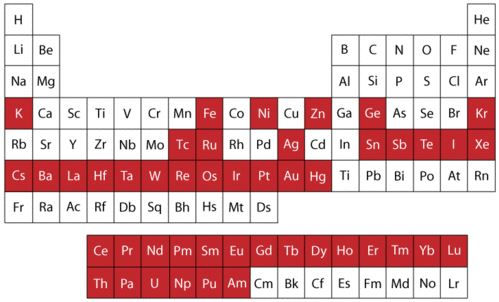
\includegraphics[width=5cm]{images/isotopes.jpg}
				\credit{Chemistry LibreTexts \cite{web:isotopes}}
				\caption{Mössbauer active elements}
			\end{figure}
		\end{block}
	\end{frame}